% !TeX root = ../beamer.tex
\section{Kreuzkorrelation in Formeln}

\begin{frame}
    \frametitle{Kreuzkorrelation}

    \begin{itemize}
        \item Gibt Aussage über \textbf{Zeitversatz} zweier Signale
        \item Definition für Referenzsignal \(x_{r}\) und Echosignal \(x_{e}\):
              \begin{equation}
                  \psi(t) = \int_{-T/2}^{T/2}{ x_{e}(s) x_{r}^{*}(s - t) \, d s}
              \end{equation}
        \item<2-> Ausgedrückt als bistatische Entfernung (\(R = c t\)):
              \begin{equation}
                  \psi(R) = \int_{-T/2}^{T/2}{ x_{e}(s) x_{r}^{*} \left( s - \frac{R}{c} \right) \, d s}
              \end{equation}
        \item<3-> Wird über \textbf{Bereich von \(R\)} ausgewertet
    \end{itemize}
\end{frame}

\begin{frame}
    \frametitle{Nächster Schritt: Kreuzambiguitätsfunktion}

    \begin{itemize}
        \item Definition:
              \begin{equation}
                  \psi(R, V) = \int_{-T/2}^{T/2} {x_{e}(s) \cdot x_{r}^{*}} \left( s - \frac{R}{c} \right)\mathrm{e}^{- \mathrm{j} \frac{2 \pi}{\lambda} V s} \, d s
              \end{equation}
        \item Berücksichtigt auch \textbf{Dopplershift} und damit bistatische Geschw.
        \item Wird über \textbf{Bereich von \(R\) und \(V\)} ausgewertet
    \end{itemize}
\end{frame}

\section{Geschichte}

\begin{frame}
    \frametitle{Das Daventry Experiment}

    \begin{columns}
        \begin{column}{0.5\textwidth}
            \begin{itemize}
                \item \textbf{Passives} Radar
                \item BBC Sendeturm als Beleuchter
                \item Detektion von Bomber-Flugzeug
            \end{itemize}
        \end{column}
        \begin{column}{0.5\textwidth}
            \begin{figure}
                \centering
                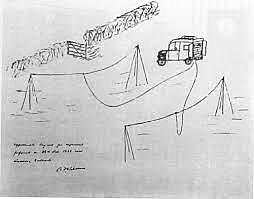
\includegraphics[width=\linewidth{},height=\textheight{}-3cm,keepaspectratio]{daventry_experiment.jpg}
                \caption{Skizze des Daventry Experiments von 1935~\cite{WattsonWatt1935}.}
            \end{figure}
        \end{column}
    \end{columns}
\end{frame}

\begin{frame}
    \frametitle{Chain Home}

    \begin{columns}
        \begin{column}{0.5\textwidth}
            \begin{itemize}
                \item Aktives Radar
                \item Nutzung während des 2. Weltkriegs
                \item Frühwarnradar gegen deutsche Luftangriffe
                \item Erste Inbetriebnahme 1937
            \end{itemize}
        \end{column}
        \begin{column}{0.5\textwidth}
            \begin{figure}
                \centering
                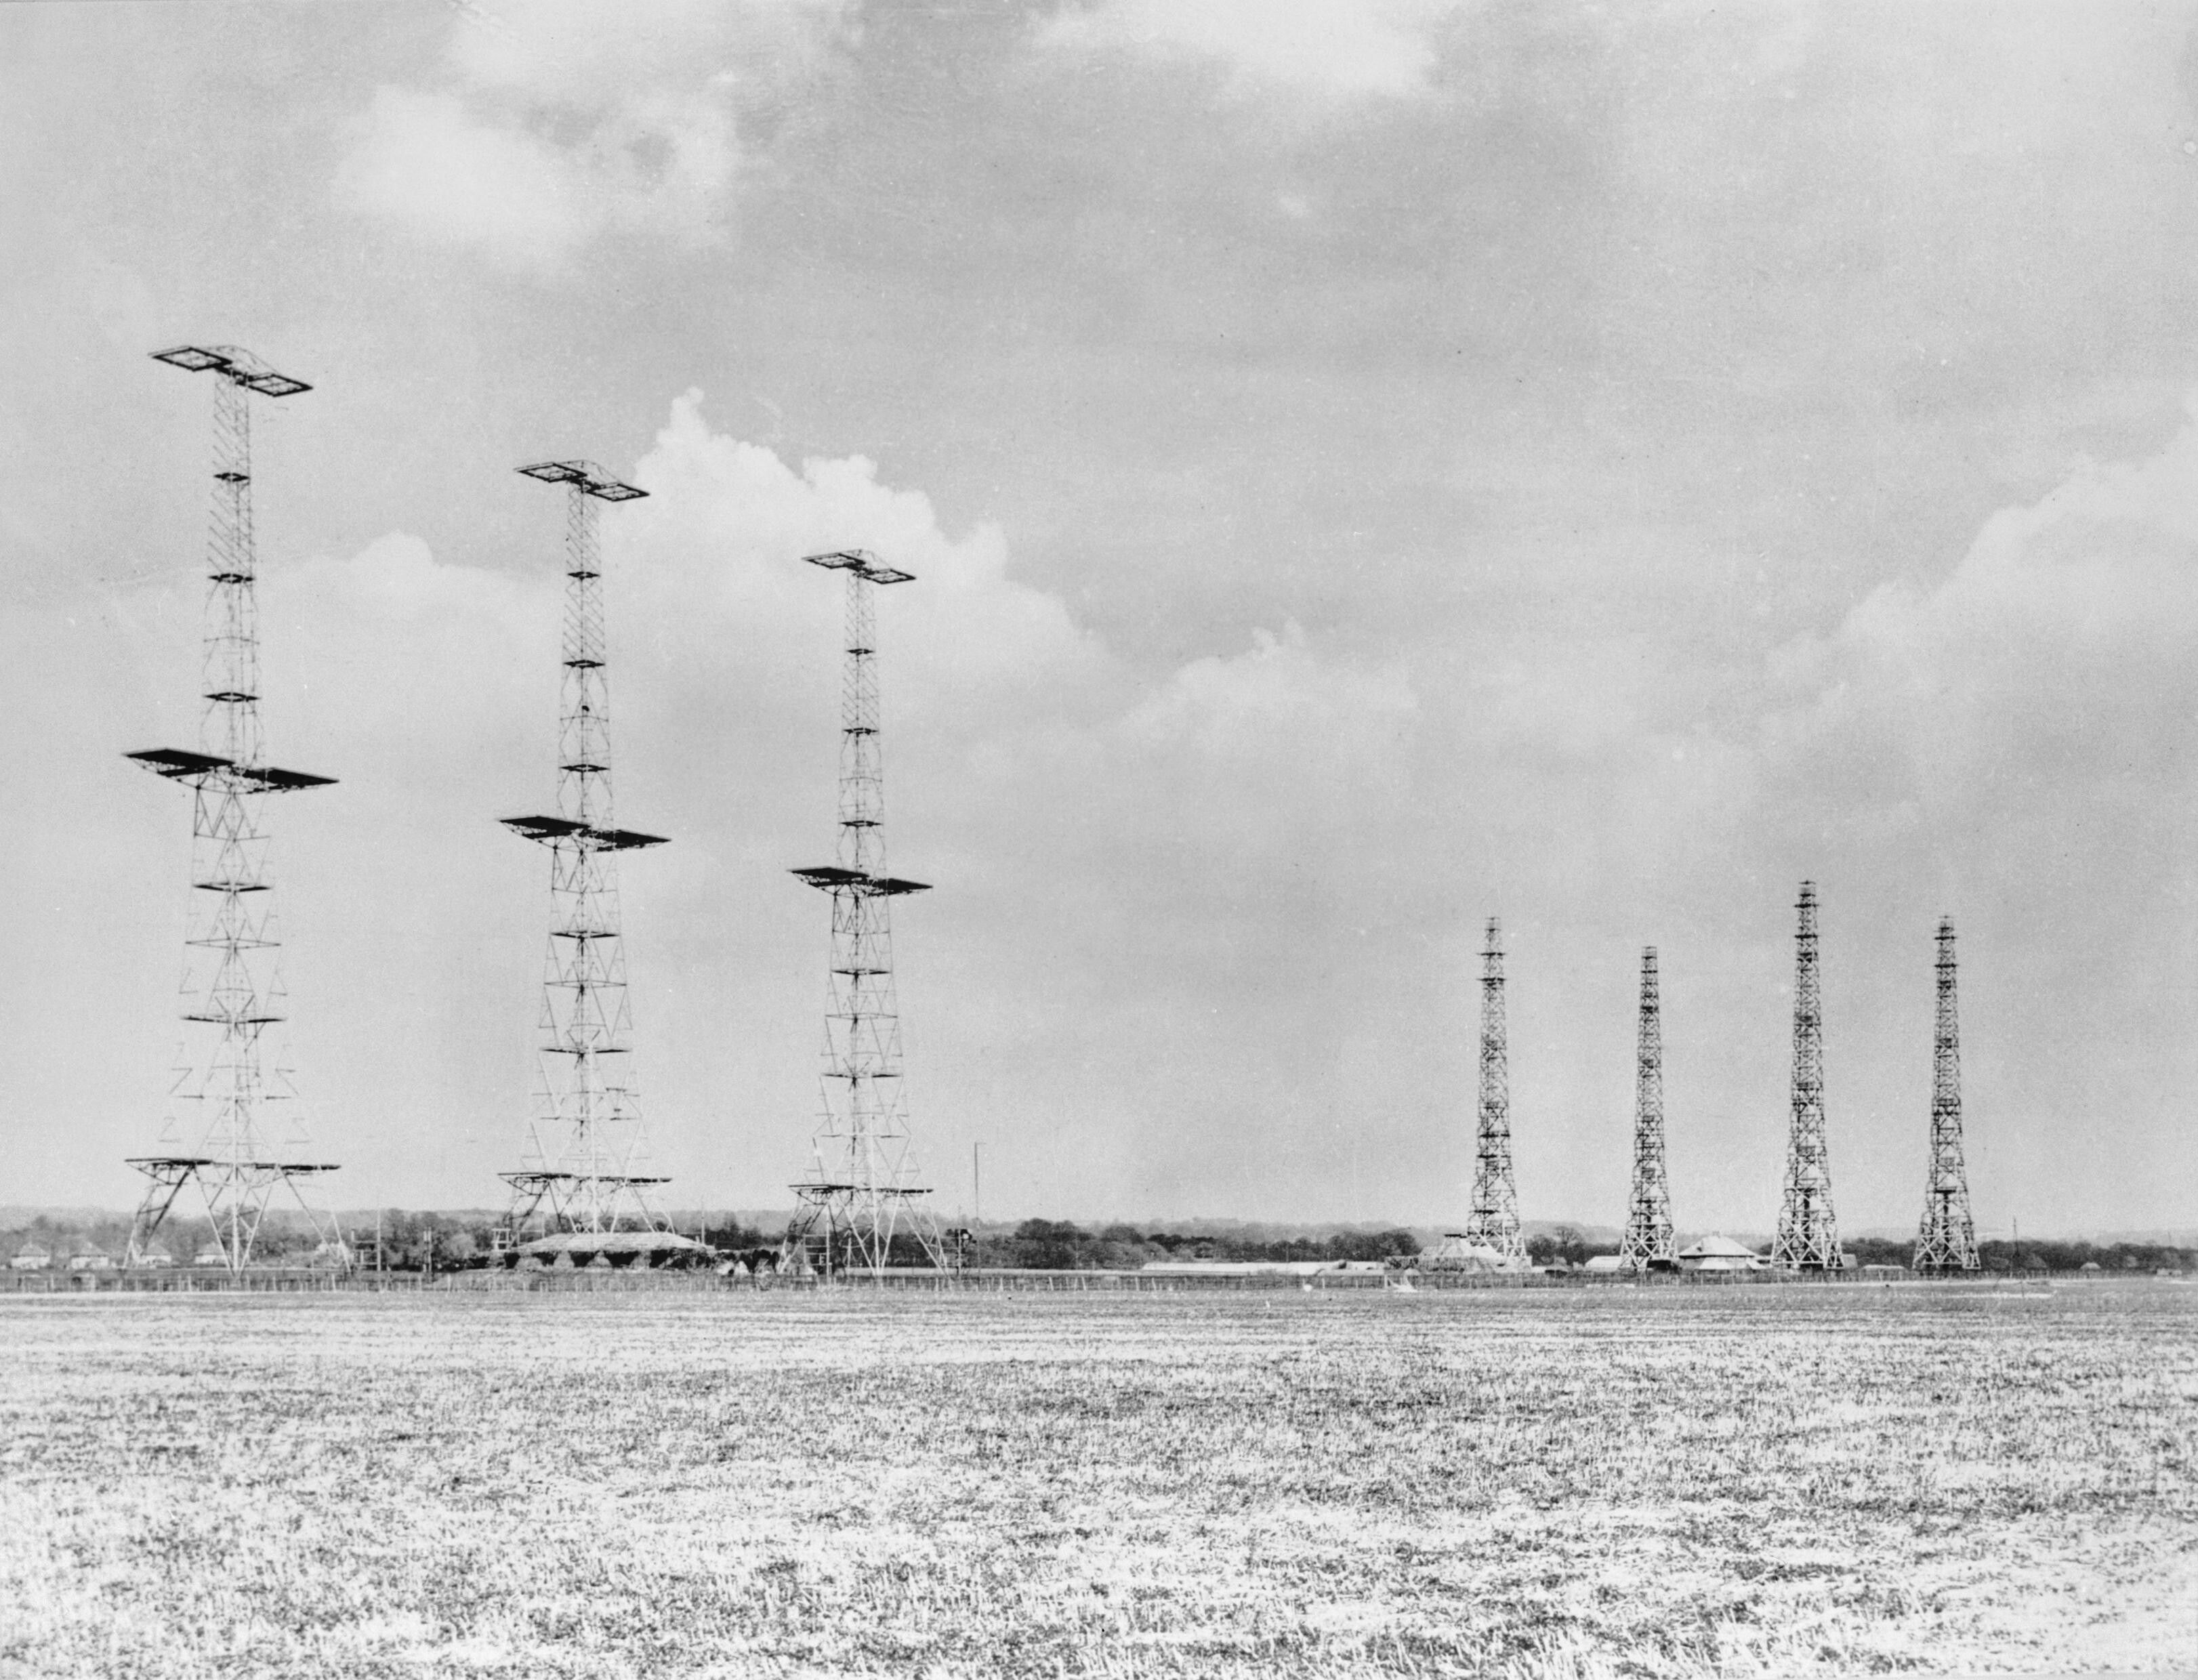
\includegraphics[width=\linewidth{},height=\textheight{}-3cm,keepaspectratio]{chain_home.jpg}
                \caption{Chain Home Antennen der Royal Airforce. Foto 1945~\cite{RoyalAirForce1945}.}
            \end{figure}
        \end{column}
    \end{columns}
\end{frame}

\begin{frame}
    \frametitle{Klein Heidelberg}

    \begin{columns}
        \begin{column}{0.44\textwidth}
            \begin{figure}
                \centering
                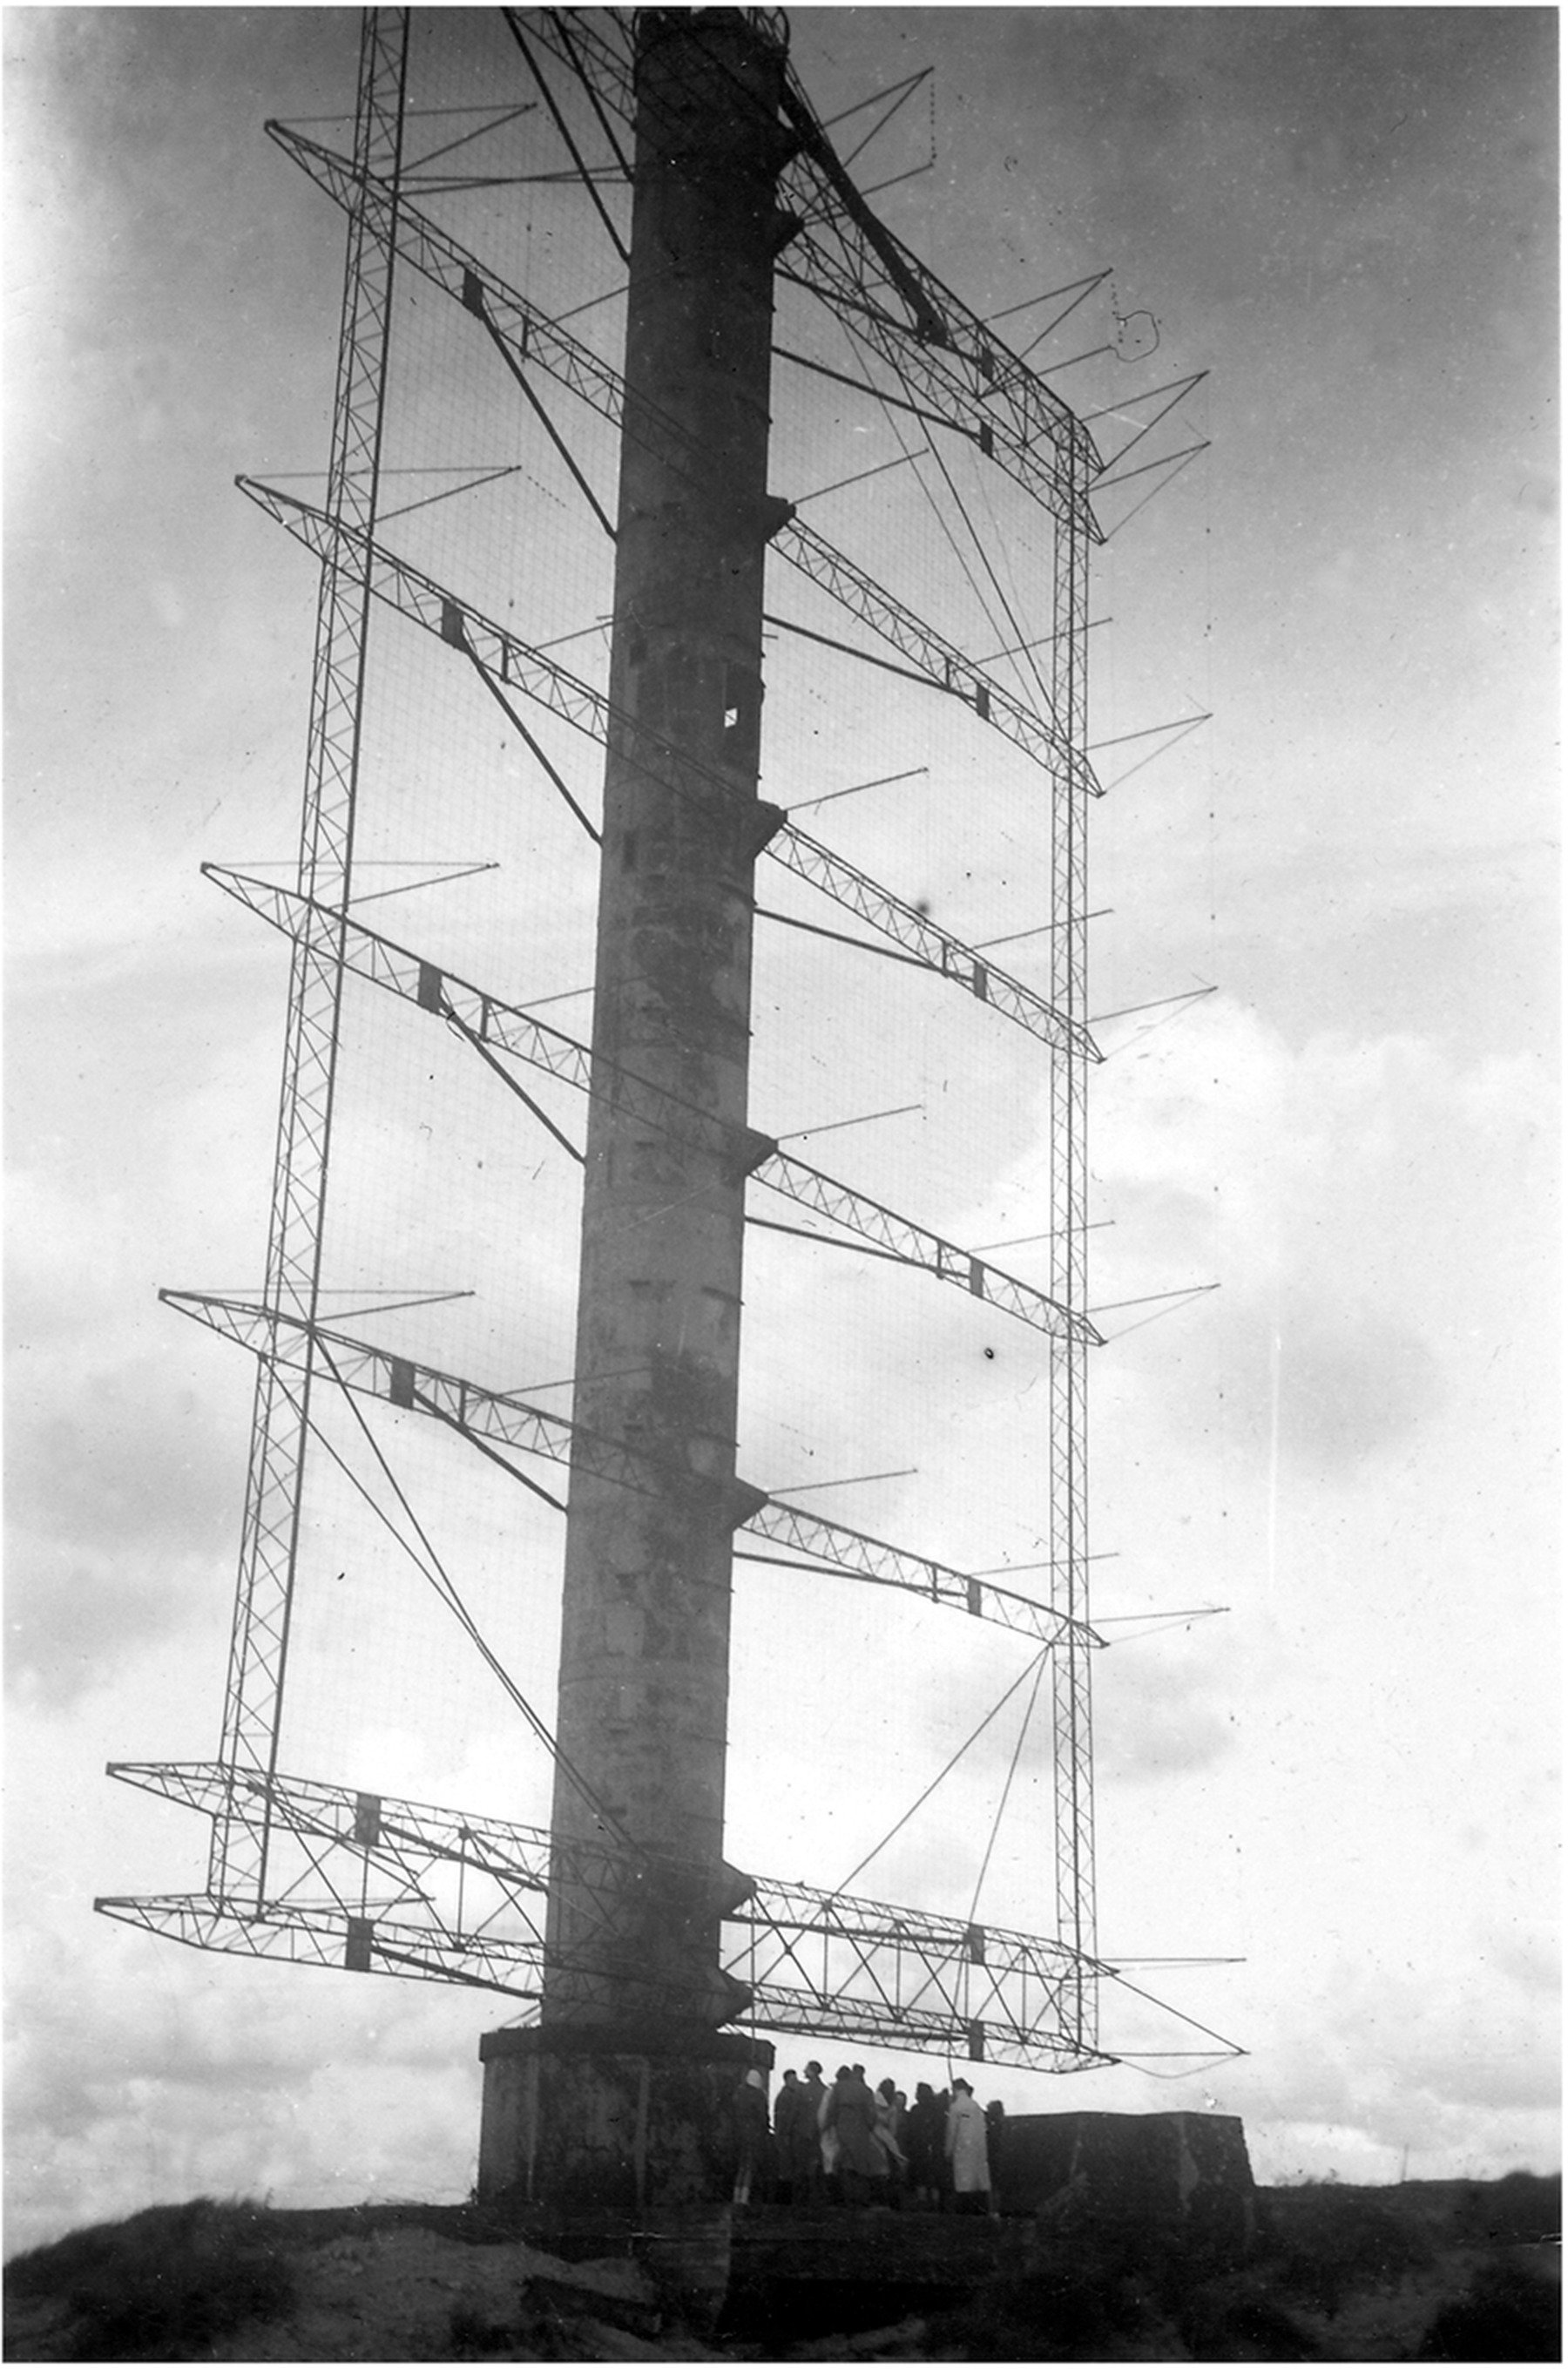
\includegraphics[width=\linewidth{},height=\textheight{}-3.5cm,keepaspectratio]{klein_heidelberg.jpg}
                \caption{Antenne des Klein Heidelberg Empfängers BIEBER (Oostvoorne, NL). Foto 1947~\cite{Rijpsma2005} as cited in~\cite{Griffiths2010}.}
            \end{figure}
        \end{column}
        \begin{column}{0.56\textwidth}
            \begin{itemize}
                \item \textbf{Passives} Radar
                \item Detektion von britischen Bombern über dem Ärmelkanal
                \item Nutzte \textbf{britisches Chain-Home} als Beleuchter
                \item Fertigstellung 1942
            \end{itemize}
        \end{column}
    \end{columns}
\end{frame}

\begin{frame}
    \frametitle{Neuzeit}

    \begin{columns}
        \begin{column}{0.55\textwidth}
            \begin{figure}
                \centering
                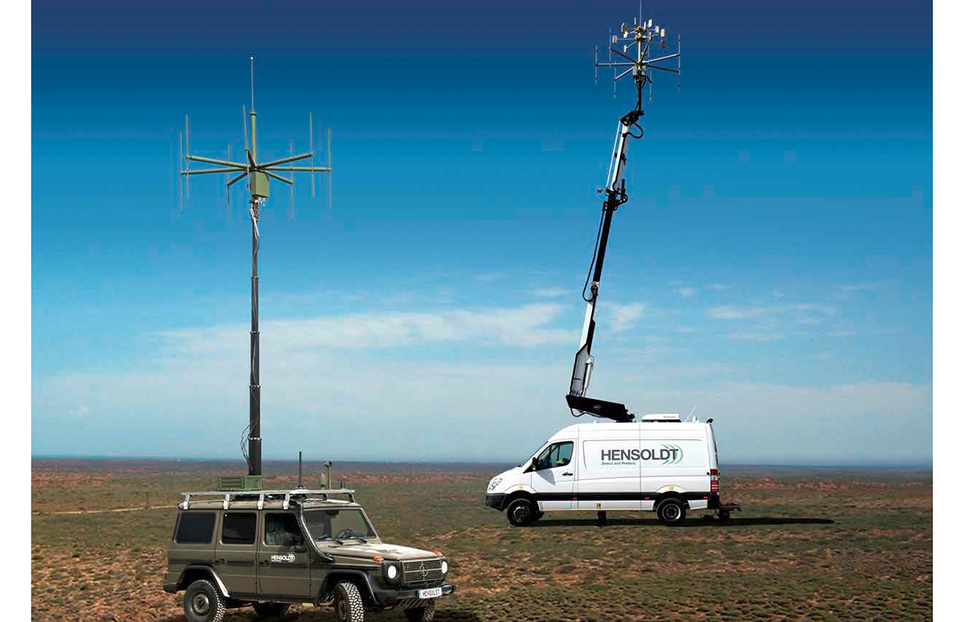
\includegraphics[width=\linewidth{},height=\textheight{}-3cm,keepaspectratio]{twinvis.png}
                \caption{TwInvis®. Modernes Passivradarsystem des Unternehmens Hensoldt~\cite{Hensoldt2019}.}
            \end{figure}
        \end{column}
        \begin{column}{0.45\textwidth}
            \begin{itemize}
                \item Zunächst basierend auf FM Beleuchtern
                \item Später DAB und DVB-T
                \item GSM, LTE
                \item \dots
            \end{itemize}
        \end{column}
    \end{columns}
\end{frame}

\section{Beleuchtungsquellen}

\begin{frame}
    \frametitle{Beleuchtungsquellen (Illuminators of Opportunity)}

    \begin{columns}
        \begin{column}{0.2\textwidth}
            \begin{figure}
                \raggedleft{}
                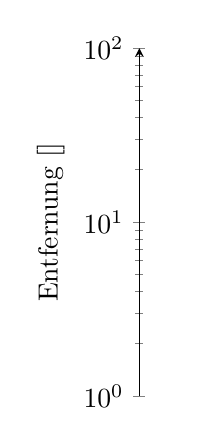
\begin{tikzpicture}
                    \begin{axis}[
                            ymode=log,
                            height=6cm,
                            width=2cm,
                            hide x axis,
                            axis y line=left,
                            ymin=1,
                            ymax=100,
                            ylabel={Entfernung [\si{\kilo\metre}]},
                        ]
                        \addplot [draw=none] {1};
                    \end{axis}
                \end{tikzpicture}
            \end{figure}
        \end{column}
        \begin{column}{0.8\textwidth}
            \begin{itemize}
                \item FM-Radio
                \item DVB-T (Digitales Fernsehen)
                \item DAB (Digitales Radio)
                \item LTE
                \item GSM
                \item WiFi
            \end{itemize}
        \end{column}
    \end{columns}
\end{frame}
